\documentclass{article}
\usepackage[utf8]{inputenc}
\usepackage{geometry}
\geometry{
  a4paper,
  total={170mm,257mm},
  left=20mm,
  top=20mm,
}
\usepackage{graphicx}
\usepackage{titling}
\usepackage{booktabs}
\usepackage{listings}
\usepackage{xcolor}
\usepackage{hyperref}
\usepackage{fancyvrb}
\usepackage{float}
\usepackage{amsmath}

\definecolor{darkblue}{rgb}{0.0, 0.0, 0.5}
\RecustomVerbatimEnvironment{verbatim}{Verbatim}{formatcom=\color{darkblue}}
\setlength{\parindent}{0pt}

\title{\textbf{Advanced Programming for HPC } \\
{\Large \textbf{Labwork 2: Get to Know Your GPU}}}
\date{Sep 2026}

\usepackage{fancyhdr}
\fancypagestyle{plain}{
  \fancyhf{}
  \fancyfoot[L]{\thedate}
  \fancyfoot[R]{\thepage}
  \fancyhead[L]{University of Science and Technology of Hanoi}
  \fancyhead[R]{Advanced Programming for HPC}
}
\makeatletter
\def\@maketitle{%
  \newpage
  \vskip 1em
  \begin{center}
  \let \footnote \thanks
    {\LARGE \@title \par}%
    \vskip 1em
  \end{center}
  \par
  \vskip 1em}
\makeatother

\begin{document}
\pagestyle{plain}
\maketitle

\noindent\begin{tabular}{@{}ll}
  Student: & Vu Ha Vy -- 2540112 \\
\end{tabular}

\section*{GPU Hardware Summary}
The execution output from Google Colab:

\begin{table}[H]
\centering
\begin{tabular}{ll}
\toprule
\textbf{Property} & \textbf{Value} \\
\midrule
Device ID & 0 \\
Device Name & Tesla T4 \\
Compute Capability & 7.5 \\
PCI Bus ID & 0 \\
PCI Device ID & 4 \\
UUID & GPU-b48a33b6-9da6-c0ba-7899-678ed7de2bda \\
Watchdog & Disabled \\
FP32/FP64 Performance Ratio & 32 \\
Multiprocessor Count (SMs) & 40 \\
Total CUDA Cores & 2560 \\
Free Memory & 15,527,116,800 bytes (14.46 GB) \\
Total Memory & 15,637,086,208 bytes (14.56 GB) \\
\bottomrule
\end{tabular}
\caption{GPU Overview}
\label{tab:gpu_specs}
\end{table}

\begin{figure}[H]
    \centering
    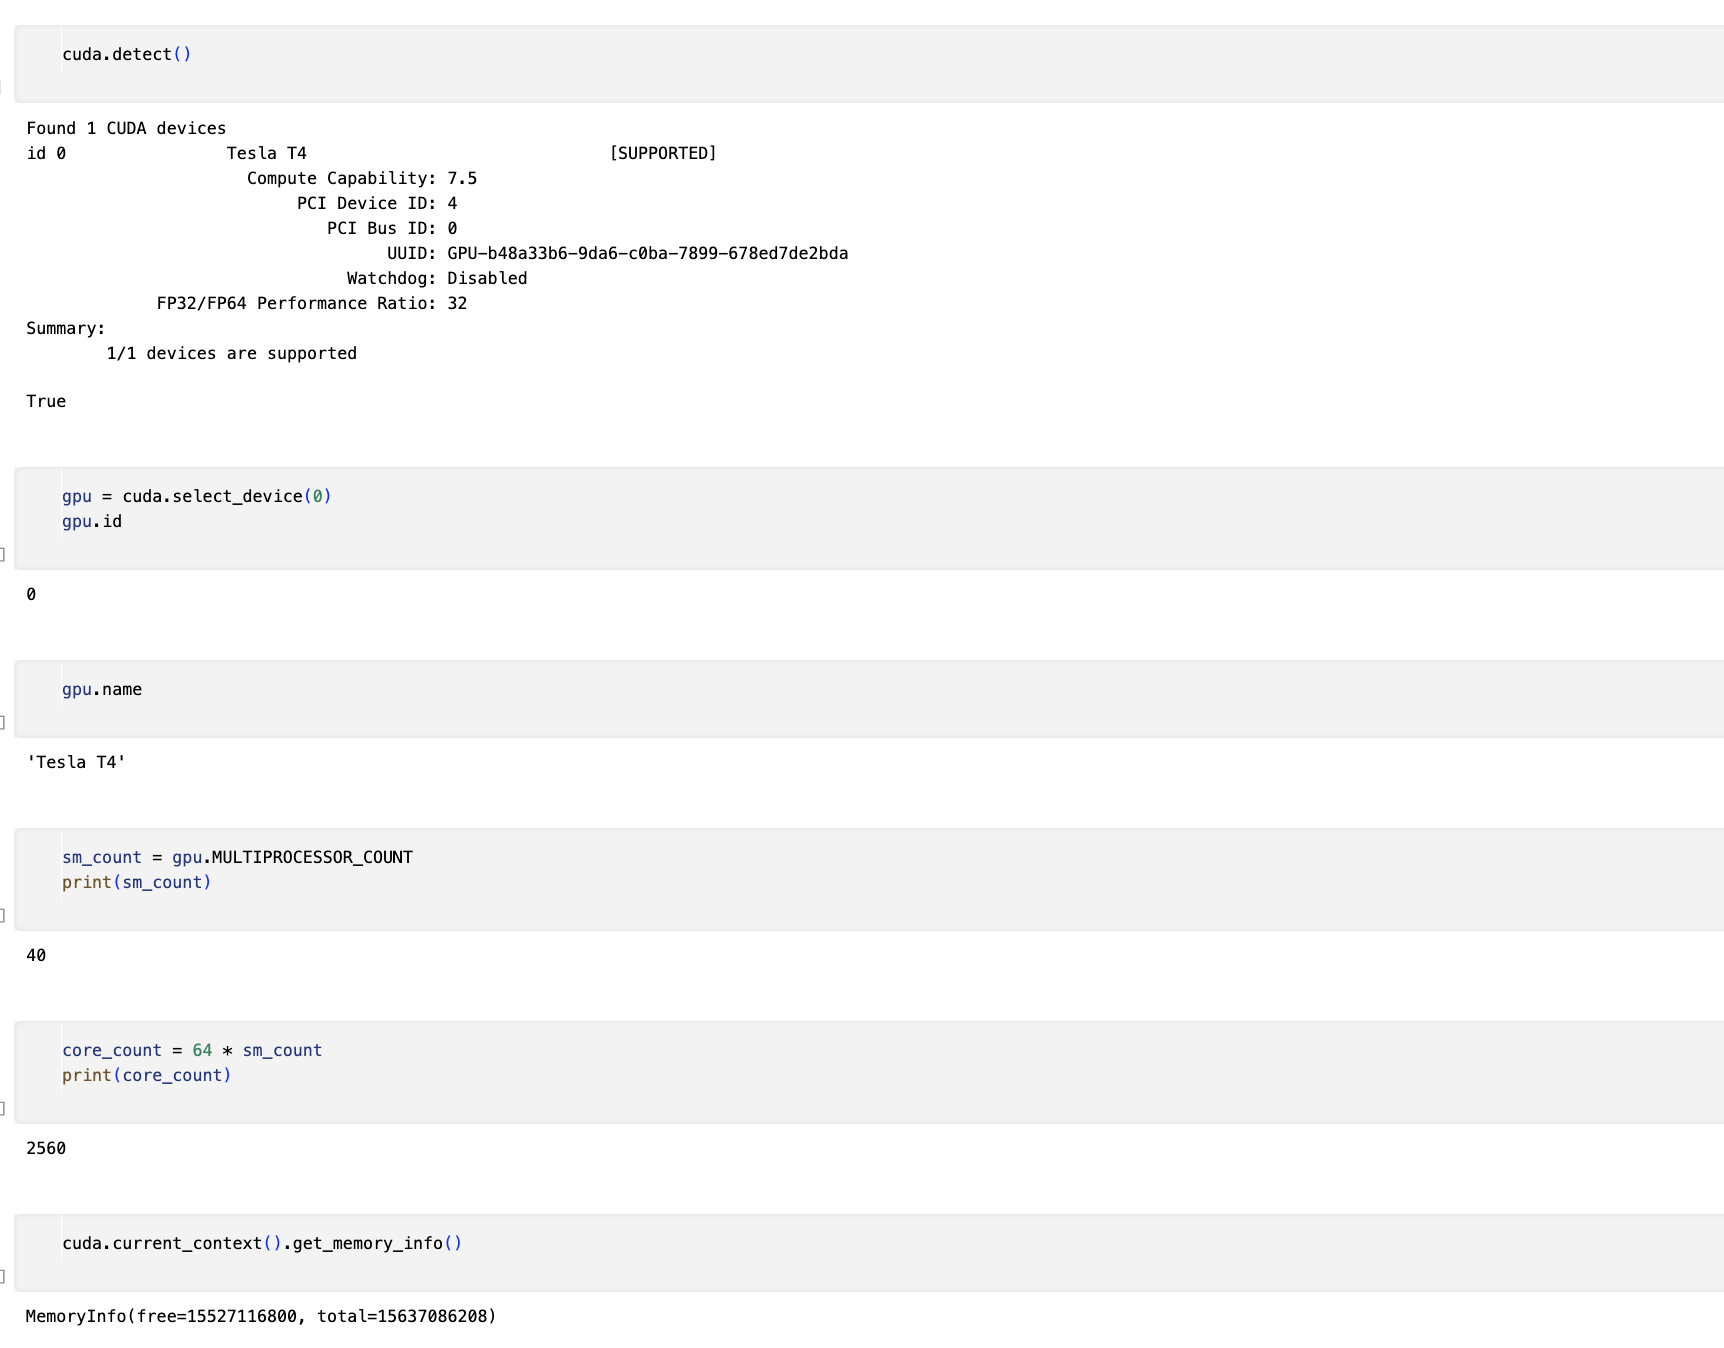
\includegraphics[width=0.85\textwidth]{report2.png}
        \caption{Captured output of the labwork.}
    \end{figure}


\end{document}